\chapter{Flight Test Data}
\label{app:flightdata}
%%%  FLYTTES TIL APPENDIX
\begin{comment}
The pilot was instructed to take-off, fly about a meter in direction, and land on a specific location. The graphs show how the entire route in z-direction. 

% Should show novice pilot data first, then say we got a pilot and did the same tests and show that data.
% - JD the animal

Fig. \ref{VPQ1zAxisTomas} shows the same ground effect tendency as in Fig. \ref{VPQzAxisTommy}. The bouncing effect seems starts to appear around 500mm above ground. 

%landing z fpq, vpq
\begin{figure}[H]
    \centering
         \includegraphics[width = 1\textwidth]{VAPIQ-PICTURES/VPQ2.jpg}
      \caption{Fixed pitch landings z-axis}
    \label{VPQ2zAxisTomas}
\end{figure} 

\begin{figure}[H]
    \centering
         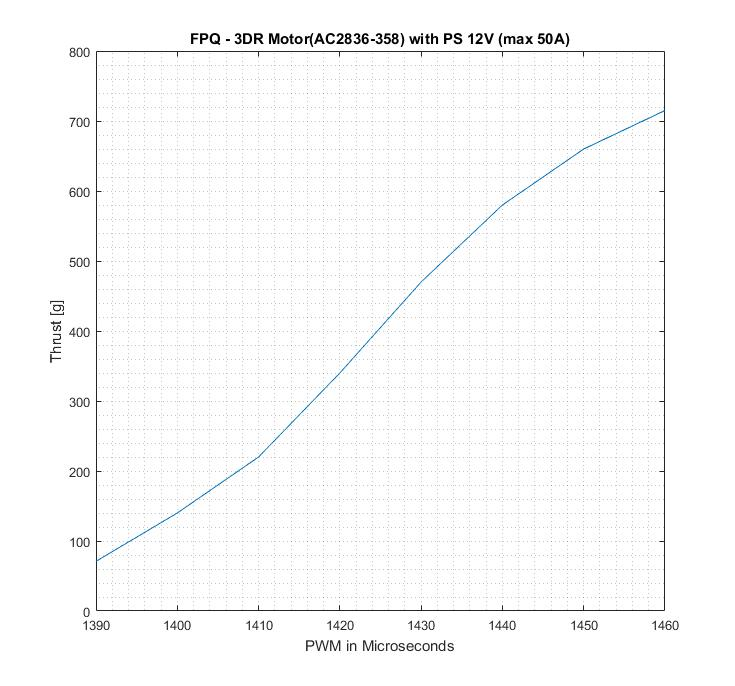
\includegraphics[width = 1\textwidth]{VAPIQ-PICTURES/FPQ1.jpg}
      \caption{Variable pitch landings z-axis}
    \label{FPQ1zAxisTomas}
\end{figure}  


%fixed and variable pitch tomas
\begin{figure}[H]
    \centering
         \includegraphics[width = 1\textwidth]{VAPIQ-PICTURES/VPQ1.jpg}
      \caption{Variable pitch landings z-axis}
    \label{VPQ1zAxisTomas}
\end{figure}   

\begin{figure}[H]
    \centering
         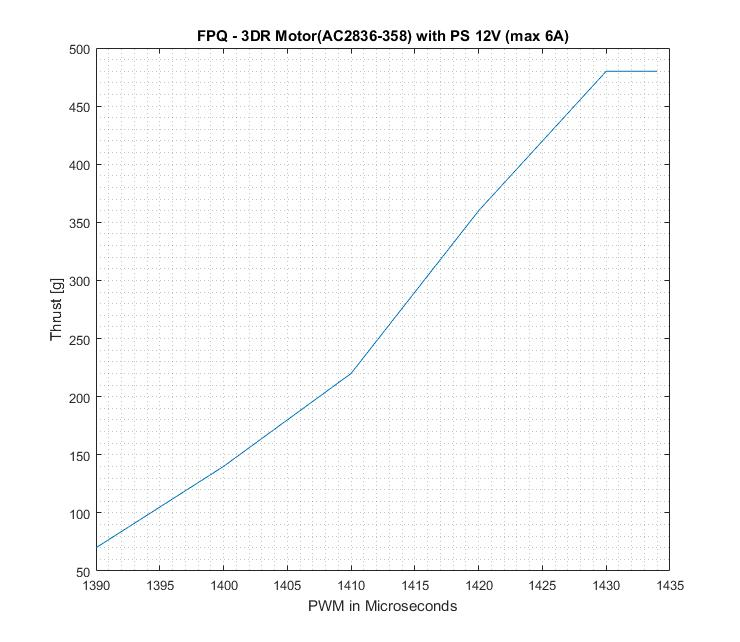
\includegraphics[width = 1\textwidth]{VAPIQ-PICTURES/FPQ2.jpg}
      \caption{Fixed pitch landings z-axis}
    \label{FPQ2zAxisTomas}
\end{figure}


%fixed and variable pitch tommy
\begin{figure}[H]
    \centering
         \includegraphics[width = 1\textwidth]{VAPIQ-PICTURES/z-axis-VPQ.jpg} % FJERN SPIKE
      \caption{Variable pitch landings z-axis}
    \label{VPQzAxisTommy}
\end{figure} 

\begin{figure}[H]
    \centering
         \includegraphics[width = 1\textwidth]{VAPIQ-PICTURES/z-axis-FPQ.jpg}
      \caption{Fixed pitch landings z-axis}
    \label{FPQzAxisTommy}
\end{figure} 

%fixed and variable pitch ground effects
\begin{figure}[H]
    \centering
         \includegraphics[width = 1\textwidth]{VAPIQ-PICTURES/FPQgeTommy.jpg}
      \caption{Fixed Pitch Landings z-axis}
    \label{FPQAxisTommy}
\end{figure}   
\begin{figure}[H]
    \centering
         \includegraphics[width = 1\textwidth]{VAPIQ-PICTURES/VPQgeTommy.jpg}
      \caption{Variable Pitch Ground Effect z-axis}
    \label{VPQzAxisTomy}
\end{figure}\bigskip


\end{comment}
%%%%%%%%%%%%%%%%%%%%%%%%%%%%%%%%%%%%%%%%%%%%%%%%%%%%%%%%%%%%%%%%%%%%%%%%%%%%